% chktex-file -2
\section{Lexical and Syntactical Analysis}

As previously mentioned, the first step during compilation or program execution is the \emph{lexical} and \emph{syntactical analysis}.
Program source text is, without previous processing, just \emph{text} i.e., a sequence of characters.
Before the computer can even begin to analyze the semantics and meaning of a program it has to first \emph{parse} the program source text into an appropriate data structure.
This is done in two steps that are closely related and often combined, the \emph{lexical analysis} performed by a \emph{lexer} and the \emph{syntactical analysis} performed by a \emph{parser}.

\subsection{Formal Syntactical Definition by a Grammar}

Just like every natural language, most programming languages also conform to a grammar.
However, grammars for programming languages most often are of type 2 or 3 in the Chomsky hierarchy, that is \emph{context-free} and \emph{regular} languages, whereas natural languages often are type 1 or 0.
\TODO{citation}
Additionally, it is not uncommon for parser writers to formally define the grammar using some notation.
Popular options include \emph{BNF}\footnote{Backus-Naur Form, named after the two main inventors~\cite{Backus1960}} and \emph{EBNF}\footnote{Extended Backus-Naur Form, an extended version of \emph{BNF} with added support for repetitions and options without relying on recursion, first proposed by Niklaus Wirth in 1977~\cite{Wirth1977} followed by many slight alterations. The version used in this paper is defined by the ISO/IEC 14977 standard.}, \TODO{emph?} the latter of which we use here.
This paper does not further explain these notations, however Listing~\ref{lst:ebnf_reference_grammar} shows a short example grammar notated using EBNF.
For reference, Appendix~\ref{apx:grammar} contains the full grammar of rush.

\TSListing[float=h, caption={Grammar for Basic Arithmetic and Relation in EBNF Notation}, label={lst:ebnf_reference_grammar}]{listings/ebnf_reference.ebnf}

\subsection{Grouping of Characters Into Tokens}

Before the syntax of a program is validated it is common to have a lexer group certain sequences of characters into \emph{tokens}.
The set of tokens a language has is the union of the set of all terminal symbols used in context-free grammar rules and the set of regular grammar rules.
For the language defined in Listing~\ref{lst:ebnf_reference_grammar} these are the four operators `+', `-', `*' and `/', and the `integer' non-terminal.

The specifics of implementing a lexer are not explored in this paper, however a basic overview is still provided.
\TODO{or will-future?}
The base principal of a lexer is to iterate over the characters of the input to produce tokens.
Depending on the target language it might however be required to scan the input using an $n$-sized window i.e., observing $n$ characters at a time.
In the case of rush this $n$ is 2, resulting in the \Verb|Lexer| struct not only storing the current character but also the next character as seen in Listing~\ref{lst:lexer}.
For clarity, Table~\ref{tbl:lexer} shows the values of \Verb|curr_char| and \Verb|next_char| during processing of the input `\Verb|1+2==3|'.
Here every row in the table represents one point in time displaying the lexer's current state.
% Listing~\ref{lst:lexer} shows the \Verb|Lexer| struct as it is defined in rush.
% The \Verb|reader| is an iterator over the input characters, the \Verb|location| saves the current index, column, and line in the source text, and the \Verb|curr_char| and \Verb|next_char| fields holds\ldots

% TODO: why does using \Verb inside caption break compilation for @MikMuellerDev
\TSListing[first line=10, last line=16, float=t, caption={The rush \texttt{Lexer} Struct Definition}, label={lst:lexer}]{deps/rush/crates/rush-parser/src/lexer.rs}

\begin{table}[h]
	\newcommand{\lexerframe}[8][]{\tikz[baseline={(frame.base)}]{
			\node(frame)[stack=6, rectangle split part fill={#2}, #1]{
				\texttt{#3}
				\nodepart{two}\texttt{#4}
				\nodepart{three}\texttt{#5}
				\nodepart{four}\texttt{#6}
				\nodepart{five}\texttt{#7}
				\nodepart{six}\texttt{#8}
			};
			% fix margin around tikzpicture
			\node[fit={(current bounding box)}, inner ysep=.5mm, inner xsep=0]{};
		}}
	\centering
	\caption{Advancing Window of a Lexer}\label{tbl:lexer}
	\begin{tabularx}{0.95\textwidth}{rCLLl}
		Calls & State                                                                                                                                                     & \colorbox{black!20}{\Verb|curr_char|} & \colorbox{black!10}{\Verb|next_char|} & Output Token  \\
		\\[-1.1em]\hline\\[-1.1em]
		0     & \lexerframe{none}{1}{+}{2}{=}{=}{3}                                                                                                                       & \Verb|None|                           & \Verb|None|                           &               \\
		0     & \lexerframe{black!10,none}{\bfseries1}{+}{2}{=}{=}{3}                                                                                                     & \Verb|None|                           & \Verb|Some('1')|                      &               \\
		0     & \lexerframe{black!20,black!10,none}{\bfseries1}{\bfseries+}{2}{=}{=}{3}                                                                                   & \Verb|Some('1')|                      & \Verb|Some('+')|                      &               \\
		1     & \lexerframe{none,black!20,black!10,none}{\color{black!50}1}{\bfseries+}{\bfseries2}{=}{=}{3}                                                              & \Verb|Some('+')|                      & \Verb|Some('2')|                      & \Verb|Int(1)| \\
		2     & \lexerframe{none,none,black!20,black!10,none}{\color{black!50}1}{\color{black!50}+}{\bfseries2}{\bfseries=}{=}{3}                                         & \Verb|Some('2')|                      & \Verb|Some('=')|                      & \Verb|Plus|   \\
		3     & \lexerframe{none,none,none,black!20,black!10,none}{\color{black!50}1}{\color{black!50}+}{\color{black!50}2}{\bfseries=}{\bfseries=}{3}                    & \Verb|Some('=')|                      & \Verb|Some('=')|                      & \Verb|Int(2)| \\
		4     & \lexerframe{none,none,none,none,black!20,black!10}{\color{black!50}1}{\color{black!50}+}{\color{black!50}2}{\color{black!50}=}{\bfseries=}{\bfseries3}    & \Verb|Some('=')|                      & \Verb|Some('3')|                      &               \\
		4     & \lexerframe{none,none,none,none,none,black!20}{\color{black!50}1}{\color{black!50}+}{\color{black!50}2}{\color{black!50}=}{\color{black!50}=}{\bfseries3} & \Verb|Some('3')|                      & \Verb|None|                           & \Verb|Eq|     \\
		5     & \lexerframe{none}{\color{black!50}1}{\color{black!50}+}{\color{black!50}2}{\color{black!50}=}{\color{black!50}=}{\color{black!50}3}                       & \Verb|None|                           & \Verb|None|                           & \Verb|Int(3)| \\
	\end{tabularx}
\end{table}

As explained in Section~\ref{sec:stages_of_compilation}, many modern language implementations have the lexer produce tokens on demand.
Thus, a lexer requires one public method called something like \Verb|next_token| reading and returning, as the name suggests, the next token.
In Table~\ref{tbl:lexer} the column on the left displays how many times the \Verb|next_token| method has been called by the parser.
In the first three rows this count is still 0, as this happens during initialization of the lexer in order to fill the \Verb|curr_char| and \Verb|next_char| fields with sensible values before the first token in requested.
The \Verb|Eq| token, composed of two `\Verb|=|' symbols, requires the lexer to advance two times before it can be returned, which is represented by the two rows in which the call count is 4.
A simplified \Verb|Token| struct definition for the example language from Listing~\ref{lst:ebnf_reference_grammar} is shown in Listing~\ref{lst:token_simple}.

\TSListing[float=h, caption={Simplified \texttt{Token} Struct Definition}, label={lst:token_simple}]{listings/token_simple.rs}

In addition to the current and next character, a lexer also has to keep track of the current position in the source text for it to provide helpful diagnostics with locations to the user.
This is done in the \Verb|location| field which is incremented every time the lexer advances to the next character.
While producing a token the lexer can then read this field once at the start and once after having read the token and save the two values in the token's span.

A special case worth mentioning are comments.
As explained later in Section~\ref{sec:constructing_a_tree}, depending on the parser, comments may be simply ignored and skipped during lexical analysis, or get their own token kind and be treated similar to string literals.

\TODO{maybe mention having spans inclusive or exclusive}

\subsection{Constructing a Tree}\label{sec:constructing_a_tree}

The parser uses the generated tokens in order to construct a tree representing the program's syntactic structure.
Depending on how the parser should be used, this can either be a \emph{Concrete Syntax Tree} (CST) or an \emph{Abstract Syntax Tree} (AST).
The former still contains information about all input tokens with their respective locations, whilst the latter only stores the abstract program structure with just the relevant information for basic analysis and execution.
Therefore, a CST is usually used for development tools like formatters and intricate linters and analyzers where it is important to preserve stylistic choices made by the programmer or to know the exact location of every token.
However, an AST is enough for interpretation and compilation as it preserves the semantic meaning of the program.
Figure~\ref{fig:parser_simple_ast} shows an AST for the program `\Verb|1+2==3|' in the language notated in Listing~\ref{lst:ebnf_reference_grammar} on page~\pageref{lst:ebnf_reference_grammar}.

\begin{wrapfigure}{R}{0.5\textwidth}
    \centering
    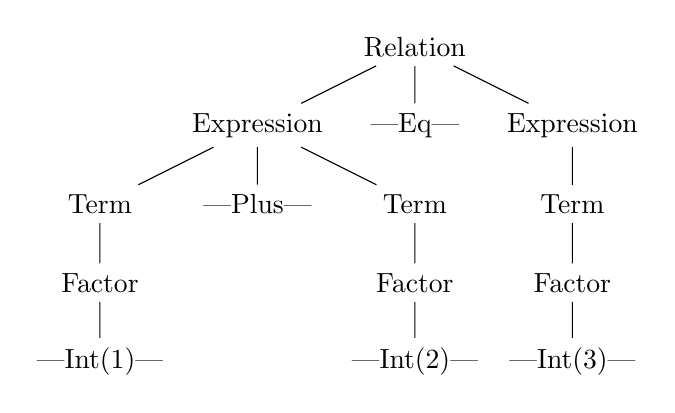
\begin{tikzpicture}[level distance=1cm, sibling distance=2cm]
        \node {Relation}
            child {node {Expression}
                child {node {Term}
                    child {node {Factor}
                        child {node {\Verb|Int(1)|}}}}
                child {node {\Verb|Plus|}}
                child {node {Term}
                    child {node {Factor}
                        child {node {\Verb|Int(2)|}}}}}
            child {node {\Verb|Eq|}}
            child {node {Expression}
                child {node {Term}
                    child {node {Factor}
                        child {node {\Verb|Int(3)|}}}}};
    \end{tikzpicture}
    \caption{Abstract Syntax Tree for `\texttt{1+2==3}'}\label{fig:parser_simple_ast}
\end{wrapfigure}

\begin{enumerate}
    \item different strategies (LL, LR) and top-down / bottom-up
    \item lookahead (to avoid backtracking)
    \item pratt-parsing
    \item parser generators
\end{enumerate}

\begin{itemize}
    \item top-down
    \begin{itemize}
        \item pre-order traversal
        \item example LL $\rightarrow$ example recursive descent
    \end{itemize}
    \item bottom-up
    \begin{itemize}
        \item post-order traversal
        \item example LR $\rightarrow$ example shift-reduce
    \end{itemize}
    \item first L means left to right
    \item second L/R means leftmost/rightmost derivation
    \begin{itemize}
        \item \TODO{explain this?}
    \end{itemize}
\end{itemize}

Just like lexers, a parser can also observe more than one token simultaniously.
This is called \emph{lookahead}.
\ldots

For most intents and purposes it is generally not recommended and necessary to implement parsers, and with that lexers, manually.
\TODO{citation}
Instead, there are so-called \emph{parser generators} that generate parsers based on some specification of the desired syntax.
Often parser generators define a domain specific grammar notation for the syntax specification.
\TODO{some also allow traditional grammar notations, and e.g., `nom' is simply a Rust crate}
\ldots
